\begin{answer}
    \begin{figure}[H]
        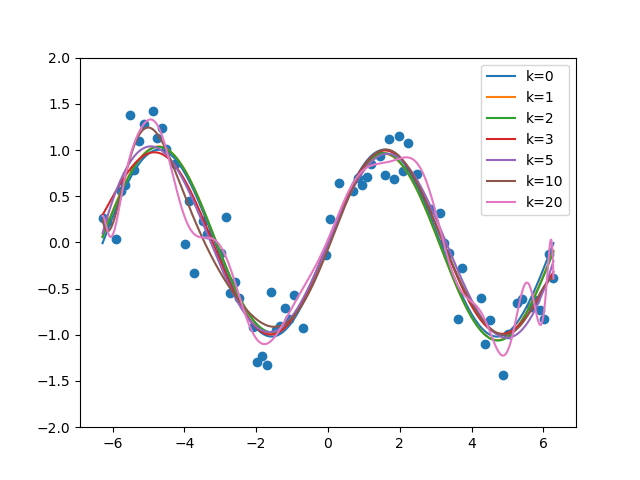
\includegraphics[width=\textwidth]{../src/featuremaps/sine.png}
        \caption{Sine and polynomial for $k=0,1,2,3,5,10,20$}
    \end{figure}
    Even in small degrees, the sine function is a better fit than the polynomial. 
    This is because the sine function captures the feature of data very well while
    the polynomial only accounts for some noise in the data, which also leads to
    overfitting when the degree is too high.
\end{answer}
